\subsection{Introduction}
This method aims to localize a vehicle at night by using a pair of images taken at different time instances (non consecutive). Unlike standard object detection methods, this approach leverages geometric reasoning and camera calibration to estimate the 3D position and orientation of the vehicle using only the taillights visible in nighttime conditions. The technique relies on identifying two pairs of corresponding symmetric points (in our case the taillights) on the rear of a moving vehicle in two non consecutive frames and applies principles from projective geometry and perspective analysis to infer spatial information.

\subsection{Methodology}

Knowing that the camera calibration matrix was previously computed, and having previously found the rear lights reference points, we define the image points as follows:
\[
\text{Left taillight: } L_1, \quad \text{Right taillight: } R_1 \quad \text{(frame 1)}
\]
\[
\text{Left taillight: } L_2, \quad \text{Right taillight: } R_2 \quad \text{(frame 2)}
\]

We then consider these image points in homogeneous coordinates:
\[
\tilde{L}_1 = \begin{bmatrix} x_{L_1} \\ y_{L_1} \\ 1 \end{bmatrix}, \quad \tilde{R}_1 = \begin{bmatrix} x_{R_1} \\ y_{R_1} \\ 1 \end{bmatrix}, \quad \tilde{L}_2 = \begin{bmatrix} x_{L_2} \\ y_{L_2} \\ 1 \end{bmatrix}, \quad \tilde{R}_2 = \begin{bmatrix} x_{R_2} \\ y_{R_2} \\ 1 \end{bmatrix}
\]

\subsubsection{Vanishing points and vehicle motion}
Two vanishing points needed for this method, are computed as:
\begin{itemize}
    \item \( V_x \): from the intersection of the taillight segments in each of the two frames:
    \[
    \ell_1 = \tilde{L}_1 \times \tilde{R}_1, \quad \ell_2 = \tilde{L}_2 \times \tilde{R}_2
    \]
    \[ \quad V_x = \ell_1 \times \ell_2
    \]
    \item \( V_y \): from the intersection of two left rear lights, and two right rear lights of the two frames:
    \[
    \ell_L = \tilde{L}_1 \times \tilde{L}_2, \quad \ell_R = \tilde{R}_1 \times \tilde{R}_2 \]
    \[\quad V_y = \ell_L \times \ell_R
    \]
\end{itemize}

These vanishing points are back-projected into the camera coordinate system using the inverse of the calibration matrix \( K \).

\[
\vec{d}_x = K^{-1} V_x, \quad \vec{d}_y = K^{-1} V_y
\]

This operation yields direction vectors, called \textit{back-projected rays}, which represent the 3D directions in space corresponding to the vanishing points observed in the image. Each ray originates from the camera center and points along the direction in which a set of 3D parallel lines project to the same vanishing point in the image. These rays are then normalized to unit vectors for the next geometric computation.

\[
\vec{d}_x = \frac{\vec{d}_x}{\|\vec{d}_x\|}, \quad \vec{d}_y = \frac{\vec{d}_y}{\|\vec{d}_y\|}
\]

The vehicle motion is assumed to be straight (no steering) if:
\[
\vec{d}_x \cdot \vec{d}_y \approx 0
\]

which we checked in our code confirming our assumption.

\subsubsection*{3D Reconstruction of rear plane and depth estimation}

% da rivedere 

To estimate the 3D position and orientation of the vehicle's rear plane, we exploit the geometric structure observed in a pair of images and the known camera calibration matrix \( K \in \mathbb{R}^{3 \times 3} \). We consider 3D world points \( \mathbf{X} \in \mathbb{R}^3 \) project onto 2D image points \( \mathbf{x} \in \mathbb{P}^2 \) according to the mapping:
\[
\tilde{\mathbf{x}} \sim K [R \, | \, t] \mathbf{X}
\]
In our case, since we are working with fixed world geometry (i.e., the rear of the car) and trying to estimate depth and orientation, we simplify the analysis to the single-camera frame and image geometry.

\paragraph{Vanishing line of the rear plane}
The vehicle’s rear is a planar surface, and it is observed in perspective, which introduces converging lines. In projective geometry, the intersection points of pairs of corresponding lines on this plane define \textbf{vanishing points} directions of parallel lines in 3D space. We identify two vanishing points:

\begin{itemize}
\item \( V_x \): from horizontal taillight edges (width-wise direction),
\item \( V_y \): from vertical motion of taillights between frames (depth-wise motion).
\end{itemize}

The \textbf{vanishing line} \( \ell \) of the rear plane is obtained as the cross product of the two vanishing points in homogeneous image coordinates:

\[
\ell = V_x \times V_y
\]

This line represents the intersection of the rear plane with the image plane, meaning it contains all the vanishing points of lines lying on the rear surface.

\paragraph{Computing the normal plane}
In projective geometry and camera imaging, every line \( \ell \) in the 2D image corresponds to a 3D plane in space that passes through the camera’s optical center and contains all the projecting rays onto that line. This is because the camera center is a fixed point in 3D space, and all points along the image line are projections of 3D points lying on some plane intersecting the camera center.

The vanishing line \( \ell \), defined as the cross product of two vanishing points \( V_x \) and \( V_y \):
\[
\ell = V_x \times V_y
\]
represents the image of the rear plane of the vehicle. Intuitively, this line corresponds to the horizon line of that plane in the image, containing all vanishing points of directions lying on the rear surface.

To determine the orientation of this plane in 3D, we back-project the image line \( \ell \) into the camera coordinate system using the transpose of the camera intrinsic matrix \( K \):
\[
\vec{n} = K^\top \ell
\]
This operation produces a vector \( \vec{n} \) that is \textbf{normal} (perpendicular) to the corresponding 3D plane in the camera coordinate frame.

\begin{figure}
    \centering
    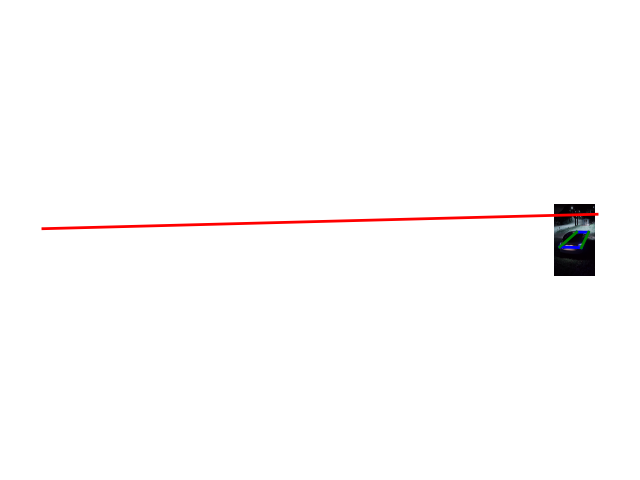
\includegraphics[width=0.75\linewidth]{Images/vanishing_line_method2.png}
    \caption{Lights segments and resulting vanishing line.}
    \label{fig:vanLine1}
\end{figure}

This result can be understood by considering the duality between points and lines in projective geometry, combined with the role of the intrinsic matrix \( K \):

\begin{itemize}
    \item The intrinsic matrix \( K \) maps a 3D direction vector \( \mathbf{d} \) expressed in the camera coordinate system to its corresponding point \( \tilde{\mathbf{p}} \) in the normalized image plane through the relation:
    \[
    \tilde{\mathbf{p}} = K \mathbf{d}
    \]
    Here, \( \tilde{\mathbf{p}} \) is a homogeneous 2D image point (or vanishing point) representing the projection of the 3D direction.

    \item Lines in the image, such as \( \ell \), are represented as vectors orthogonal to points (in the dual projective space). When we want to find the 3D plane corresponding to an image line, we need to "lift" this line back into 3D space.

    \item The transpose \( K^\top \) operates on image lines \( \ell \) to map them back into 3D vectors normal to the planes whose images they represent. More formally, since \( \ell \) satisfies \( \ell^\top \tilde{\mathbf{p}} = 0 \) for all points \( \tilde{\mathbf{p}} \) on that line, applying \( K^\top \) to \( \ell \) produces a vector \( \vec{n} \) such that:
    \[
    \vec{n}^\top \mathbf{d} = 0
    \]
    for all directions \( \mathbf{d} \) whose image points lie on \( \ell \).

    Thus, \( \vec{n} = K^\top \ell \) defines the normal vector to the 3D plane associated with the image line \( \ell \).
\end{itemize}


Since \( \vec{n} \) is defined up to scale, it is normalized to obtain a unit normal vector:
\[
\vec{n} = \frac{\vec{n}}{\|\vec{n}\|}
\]

The normalized vector \( \vec{n} \) thus precisely encodes the orientation of the vehicle’s rear plane relative to the camera frame. It points orthogonally outward from the rear surface, enabling further computations such as projecting points onto the plane or estimating distances from the camera.


\paragraph{Back-projected rays to the taillights}

Next, we compute the direction vectors from the camera center to the left and right taillights in the image. These are known as \textbf{back-projected rays}, obtained by applying the inverse of the calibration matrix to the image points:

\[
\vec{r}_{L_1} = \frac{K^{-1} \tilde{L}_1}{\|K^{-1} \tilde{L}_1\|}, \quad 
\vec{r}_{R_1} = \frac{K^{-1} \tilde{R}_1}{\|K^{-1} \tilde{R}_1\|}
\]

Each ray represents the direction in 3D along which a taillight lies, assuming the scene is rigid and the taillight is a fixed point in the world.

\paragraph{Angle between rays and depth estimation}

Given these rays, the angular separation between them in 3D space encodes information about the apparent size of the taillight segment. The angle \( \theta \) between the rays is computed via the dot product:

\[
\cos(\theta) = \vec{r}_{L_1} \cdot \vec{r}_{R_1}, \quad 
\theta = \arccos(\cos(\theta))
\]

This angle tells us how "wide" the taillight separation appears from the camera’s point of view. Given the \textbf{real-world width} \( w \) between the taillights (e.g., from CAD data), we can apply a simple geometric principle to estimate the depth \( d \) of the car's rear from the camera:

\[
d = \frac{w}{2 \sin(\theta / 2)}
\]

This formula arises from the \textbf{law of sines} in triangle geometry. The rays \( \vec{r}_{L_1} \) and \( \vec{r}_{R_1} \) define a triangle with a known base \( w \) and angle \( \theta \) at the vertex (camera center). The depth \( d \) corresponds to the distance from the camera to the base of the triangle, projected along the median ray.

\subsubsection{3D reconstruction and bounding box}

3D coordinates of the taillights:
\[
\vec{P}_{L_1} = d \cdot \vec{r}_{L_1}, \quad \vec{P}_{R_1} = d \cdot \vec{r}_{R_1}
\]

The midpoint between taillights is:
\[
\vec{C}_{\text{rear}} = \frac{\vec{P}_{L_1} + \vec{P}_{R_1}}{2}
\]

The rear ground contact point is computed by shifting vertically:
\[
\vec{C}_{\text{ground}} = \vec{C}_{\text{rear}} + h \cdot \vec{n}
\]
where \( h \) is the taillight height from the ground.

The local coordinate frame of the vehicle is defined as:
\[
\text{Forward: } \vec{f} = \vec{d}_y \] \[\text{right: } \vec{r} = \frac{\vec{r}_{R_1} - \vec{r}_{L_1}}{\|\vec{r}_{R_1} - \vec{r}_{L_1}\|} \]

\[\text{up: } \vec{u} = \vec{n}
\]

Using the vehicle’s CAD dimensions (length \( l \), width \( w \), height \( h \)), we are able to construct the 8 corners of the 3D bounding box.

\subsubsection{Projection and visualization}

Each 3D corner \( \vec{P}_i \) is projected into 2D image space as:
\[
\tilde{p}_i = K \vec{P}_i, \quad p_i = \left( \frac{\tilde{p}_i[0]}{\tilde{p}_i[2]}, \frac{\tilde{p}_i[1]}{\tilde{p}_i[2]} \right)
\]

Figure~\ref{fig:method2_result} shows the final result of the pose estimation using only rear taillight cues under nighttime conditions.

\begin{figure}[H]
    \centering
    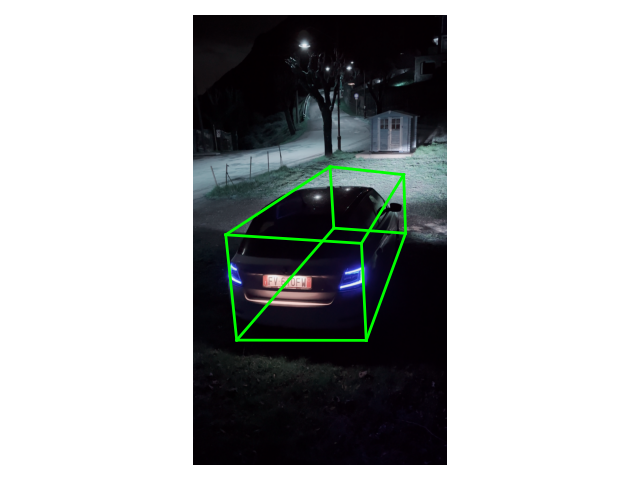
\includegraphics[width=0.75\linewidth]{bb_method2.png}
    \caption{Bounding box resulting from method 2}
    \label{fig:method2_result}
\end{figure}